\documentclass[runningheads]{llncs}
\usepackage{graphbox,graphicx}
\usepackage[labelfont=bf]{caption}
\usepackage{color}
\usepackage{subcaption}
\usepackage{booktabs}
\usepackage{multirow}
\usepackage[utf8]{inputenc}
%\usepackage{fourier} 
\usepackage{array}
\usepackage{makecell}
\usepackage{listings}
\usepackage{hyperref}
\usepackage{scalerel}
\usepackage{float}
\usepackage{amsmath, amssymb, calrsfs, wasysym, verbatim, bbm, color, graphics, geometry} %amsthm
\usepackage{bm}
\usepackage{cite}
%\usepackage{subfigure}
\graphicspath{ {./images/} }
\usepackage{tabularx}
\usepackage{enumitem}
\setlist[itemize]{leftmargin=40pt}
\usepackage{subcaption}

%\lstset{
%	basicstyle=\scriptsize\ttfamily,
%	columns=fullflexible,
%	frame=single,
%	moredelim=[is][\itshape]{[*}{*]},
%	breaklines=true,
%	breakindent=0pt
%}

\newcommand{\todo}[1]{}
\renewcommand{\todo}[1]{{\color{red}{#1}}}

\newcommand{\customsymbol}[1]{\scalerel*{\includegraphics{#1}}{`}}
\begin{document}

%\title{An Experimental Study for Federated Online Learning to Rank with Evolution Strategies}

\title{Federated Online Learning to Rank with Evolution Strategies: A Reproducibility Study}


%
%\author{You You\inst{1}\orcidID{} \and
%		Guido Zuccon\inst{1}\orcidID{0000-0003-0271-5563} \and
%		XX\inst{1}\orcidID{} \and
%		XX\inst{1}\orcidID{}}

%\institute{The University of Queensland, St Lucia, Australia}


\maketitle

\begin{abstract}
Online Learning to Rank (OLTR) optimizes ranking models using implicit users' feedback, such as clicks, directly manipulating search engine results in production. This process requires OLTR methods to collect user queries and clicks; current methods are not suited to situations in which users want to maintain their privacy, i.e. not sharing data, queries and clicks. 

Recently, the federated OLTR with evolution strategies (FOLTR) method has been proposed to provide a solution that can meet a number of users' privacy requirements. Specifically, this method exploits the federated learning framework and $\epsilon$-local differential privacy. However, the original research study that introduced this method only evaluated it on a small LTR dataset and with no conformity with respect to current OLTR evaluation practice. It further did not explore specific parameters of the method, such as the number of clients involved in the federated learning process, and did not compare FOLTR-ES with the current state-of-the-art OLTR method. This paper aims to remedy to this gap. 

Our findings question whether FOLTR-ES is a mature method that can be considered in practice: its effectiveness largely varies across datasets, click types, ranker types and settings. Its performance is also far from that of current state-of-the-art OLTR, questioning whether the maintained of privacy guaranteed by FOLTR-ES is not achieved by seriously undermining search effectiveness and user experience. 

%A recent work by Kharitonov~\cite{kharitonov2019federated} proposes a learning algorithm called FOLtR-ES that conducts Federated Machine Learning paradigm into OLTR in order to provide a solution in user privacy guarantees. This work develops a privatization procedure to guarantee $\epsilon$-local differential privacy.

%Our experiments study the reproducibility of FOLtR-ES using MSLR-WEB10K and Yahoo! Webscope datasets. For a better study in performance of FOLtR-ES comparing to other widely-used OLTR methods, we train Pairwise Differentiable Gradient Descent (PDGD) models as baselines. We also extend the online optimization metric to Discounted Cumulative Gain and use nDCG as evaluation metric to study the consistency of ranking performance in FOLtR-ES. Our experiments show FOLtR-ES can generalise on larger datasets and other common online metric. Although FOLtR-ES preserves users' privacy to some degree, it lags behind the OLTR baseline in terms of ranking performance. 

	\keywords{Online learning to rank; Federated machine learning; Differential privacy}
\end{abstract}


\section{Introduction}

one sentence for federated learning\\
\\
The following research questions are addressed in this paper:\\
\\
RQ1. Does the Federated Online Learning to Rank algorithm also work on other widely used Learning to Rank datasets?\\
RQ2. Does the number of clients affect the performance of Federated Online Learning to Rank?\\
RQ3. Can federated online learning to rank achieve similar performance comparing with other state-of-the-art online learning to rank methods?\\
RQ4. Can Federated Online Learning to Rank generalise to other typical OLTR evaluation setup, such as nDCG or MRR?\\


\section{Federated OLTR with Evolution Strategies}\label{sec:method}

We provide a brief overview of the FOLtR-ES method, which extends online LTR to federated learning; this is done by exploiting evolution strategies optimization, a widely used paradigm in Reinforcement Learning. 
The FOLtR-ES method consists of three parts. First, it casts the ranking problem into the federated learning optimization setting. Second, it uses evolution strategies to estimate gradients of the rankers. Finally, it introduces a privatization procedure to further protect users' privacy.

\subsection{ Optimization Scenario}
The optimization scenario can be illustrated as several steps. First, the client downloads the most recently updated ranking model from the server. After $B$ interactions is performed by the client, the performance metrics of the these interactions are averaged in the client side and a privatized message is sent to the centralized server. After receiving messages from $N$ clients, the server combines them to estimate a single gradient g and performs an optimization step to update the current ranking model. Finally, the clients download the newly updated model from the server.

\subsection{Gradient Estimation}
Assume that the ranking model comes from a parametric family indexed by vector $\theta \in R^{n}$. Each time a user $u$ has an interaction $a$, the ranking quality is denoted as $f$. The goal of optimization is to find model vector $\theta^*$ that can maximize the mean of metric $f$ across all interactions $a$ from all users $u$:
\begin{equation}
	\theta^{*}=\arg \max _{\theta} F(\theta)=\arg \max _{\theta} \mathbb{E}_{u} \mathbb{E}_{a \mid u, \theta} f(a ; \theta, u)
\end{equation}
By using Evolution Strategies (ES)~\cite{salimans2017evolution}, FOLtR-ES algorithm considers a population of parameter vectors which follow the distribution with a density function $p_{\phi}(\theta)$. The objective turns to finding the distribution parameter $\phi$ that can maximize the expectation of metrics across the population:
\begin{equation}
	 \mathbb{E}_{\theta\sim p_{\phi}(\theta)}~[F(\theta)]
\end{equation}
The gradient $g$ of Equation (2) is obtained in a fashion similar to REINFORCE~\cite{williams1992simple}:
\begin{equation}
	\begin{aligned}
		g &=\nabla_{\phi} \mathbb{E}_{\theta}[F(\theta)]=\nabla_{\phi} \int_{\theta} p_{\phi}(\theta) F(\theta) d \theta=\int_{\theta} F(\theta) \nabla_{\phi} p_{\phi}(\theta) d \theta=\\
		&=\int_{\theta} F(\theta) p_{\phi}(\theta)\left(\nabla_{\phi} \log p_{\phi}(\theta)\right) d \theta=\mathbb{E}_{\theta}\left[F(\theta) \cdot \nabla_{\phi} \log p_{\phi}(\theta)\right]
	\end{aligned}
\end{equation}
Same as Evolution Strategies, FOLtR-ES instantiates population distribution $p_{\phi}(\theta)$ as an isotropic multivariate Gaussian distribution with mean $\phi$ and fixed diagonal covariance matrix $\sigma^2I$. Thus a simple form of gradient estimation is denoted as:
\begin{equation}
	g=\mathbb{E}_{\theta \sim p_{\phi}(\theta)}\left[F(\theta) \cdot \frac{1}{\sigma^{2}}(\theta-\phi)\right]
\end{equation}
Based on federated optimization scenario, $\theta$ is sampled independently on client side. Combined with the definition of $F(\theta)$ in Equation (1), the gradient can be obtained as:
\begin{equation}
	g=\mathbb{E}_{u} \mathbb{E}_{\theta \sim p_{\phi}(\theta)}\left[\left(\mathbb{E}_{a \mid u, \theta} f(a ; \theta, u)\right) \cdot \frac{1}{\sigma^{2}}(\theta-\phi)\right]
\end{equation}
To get the estimate $\hat{g}$ of $g$ from Equation (5), $\hat{g} \approx g$, following steps are adopted: (a) each client $u$ randomly generates a pseudo-random seed $s$ and uses the seed to sample a perturbed model $\theta_{s} \sim \mathbb{N}\left(\phi, \sigma^{2} I\right)$, (b) uses the average of metric $f$ over $B$ interactions to estimate the expected loss $\hat{f} \approx \mathbb{E}_{a \mid u, \theta_{s}} f(a;\theta_s, u) $ from Equation (5), (c) communicates the message tuple $(s,\hat{f})$ to the server, (d) the centralized server can get the estimate $\hat{g}$ of Equation (5) according to all message sent from $N$ clients.

To reduce the variance of gradient estimates, means of antithetic variates are used in FOLtR-ES, which is also a ES trick~\cite{salimans2017evolution}. The algorithm in gradient estimation follows standard ES except that the random seeds are sampled in client side.

\subsection{Privatization Procedure}
To ensure that the clients' privacy is fully protected, FOLtR-ES proposes a privatization procedure that introduces privatization noise in the communication procedure  between clients and the server.

Assume that the metric used on client side is discrete or can be discretized if continuous. Thus the metric takes a finite number ($n$) of values, $f_0, f_1, ..., f_{n-1}$. For each time the client experiences interaction, the true value of the metric is denoted as $f_0$ and the rest of $n-1$ values are different from $f_0$. In privatization procedure, true metric value $f_0$ is sent with probability $p$. Otherwise, with probability $1-p$, send the randomly selected value $\hat{f}$ out of the remaining $n-1$ values. To ensure the same optimization goal described in section 3.3, FOLtR-ES assumes that the probability $p > 1/n$.

Unlike other Federated Learning work, FOLtR-ES adopts a strict notion of $\epsilon$-local differential privacy~\cite{}, in which the privacy is considered at the level of client side instead of the server. Through the privatization procedure, $\epsilon$-local differential privacy is achieved. And the upper bound of $\epsilon$ is:
\begin{equation}
	\epsilon \leq log\frac{p(n-1)}{1-p} 
\end{equation}
This means through the privatization scheme, at least log[$p(m-1)/(1-p)$]-local differential privacy can be achieved. At the same time, any $\epsilon$-local differential private mechanism also can obtain $\epsilon$-differential privacy~\cite{dwork2014algorithmic}.

\section{Experimental Settings}

In this section, we introduce the experimental settings to answer the research questions addressed in Section. 1.

\subsection{Datasets}
The datasets we use are MQ2007 and MQ2008~\cite{DBLP:journals/corr/QinL13}, MLSR-WEB10K\cite{DBLP:journals/corr/QinL13} and Yahoo! Webscope~\cite{DBLP:journals/jmlr/ChapelleC11} datasets, which are commonly-used offline learning to rank datasets. Each dataset contains a centain amount of queries and corresponding candidate documents. The query-document pairs are represented by feature vectors and relevance labels. For MQ2007 and MQ2008 datasets, the relevance labels value as 0 (not relevant), 1 (partially relevant) and 2 (perfecly relevant). The relevance annotations of MLSR-WEB10K range from 0 (not relevant) to 4 (perfectly relevant). Each dataset contains five splits, except for Yahoo! Webscope. More detailed information for each dataset can be found in Table \ref{table:1:dataset}.

%MQ2007 dataset contains 1692 unique queries and 69623 relevance labels. MQ2008 dataset contains 784 unique queries and 15211 relevance labels. For MQ2007 and MQ2008 dataset, each query-document pair contains 46 features.
We use the original dataset in training and validating procedure without any preprocessing, such as feature selection or feature normalization.

\begin{table}
	\caption{Information for each dataset}
	\label{table:1:dataset}
	\centering
	\begin{tabular}{l c c c}
		%\lsptoprule
		\hline
		& & number of & \\
		& queries&  relevance labels  & features \\
		\midrule
		MQ2007  &   1692  &    69623  &    46    \\
		%\hline
		MQ2008  &  784  &   15211  &    46    \\
		%\hline
		MLSR-WEB10K  &   XXX &   XXX  &    136  \\
		%\lspbottomrule
		\hline
	\end{tabular}
\end{table}

\subsection{Simulation}

Because no public datasets with search log is available for online learning to rank, we adopt the similar setup with~\cite{DBLP:conf/wsdm/SchuthOWR16, DBLP:conf/wsdm/HofmannSWR13} - simulating users and their reaction to the search results using labelled offline learning to rank datasets.

We follow the same method with FOLtR-ES for simulation. We sample $B$ queries for each client randomly and use the local perturbed model to rank the documents. The length for each ranking list is limited to 10 documents. After simulating user's clicks data, we record the quality metric for each interaction and perform the privatization procedure with probability $p$. Next, we send the averaged metric and pseudo-random seed to optimize the centralized ranking model. Finally, each client receive the updated ranking model. 

For users' click simulation, we use Cascade Click Model (CCM)~\cite{DBLP:conf/wsdm/GuoLW09}. We run instances of CCM using the same click probability and stop probability with~\cite{kharitonov2019federated} for MQ2007 and~\cite{oosterhuis2016probabilistic} for MLSR-WEB10K. Under CCM, users are assumed to go through the ranking list from top to bottom. Each document is examined and clicked with click probability $P(click = 1 | r)$, conditioned on relevance label $r$. After a click, the user stops with stop probability $P(stop = 1 | r)$ or continues otherwise. Usually three instantiations of CCM are considered in OLTR: a $perfect$ user with very reliable feedback, a $navigational$ user searching for reasonably relevant documents, and an $informational$ user with noisiest feedback among three instantiations.  table 2 shows the parameters of three click models.

\begin{table}
	\caption{Three click model instantiations for MQ2007 dataset}
	\label{table:1:dataset}
	\centering
	\begin{tabular}{l c c c}
		%\lsptoprule
		\hline
		& & number of & \\
		& queries&  relevance labels  & features \\
		\midrule
		MQ2007  &   1692  &    69623  &    46    \\
		%\hline
		MQ2008  &  784  &   15211  &    46    \\
		%\hline
		MLSR-WEB10K  &   XXX &   XXX  &    136  \\
		%\lspbottomrule
		\hline
	\end{tabular}
\end{table}


\subsection{Evaluation metric}

\subsection{Baselines}


\subsection{Models}

\subsection{Click Models}
we simulate uses by applying an instance of Cascade Click Model (CCM)~\cite{}

(further explain about CCM)

(table for CCM we use)



\section{Results and Analysis}


\subsection{RQ1: Generalisation of FOLTR-ES performance beyond MQ2007/2008}
For answering RQ1 we replicate the results obtained by Kharitonov~\cite{kharitonov2019federated} on the MQ2007 and MQ2008 datasets; we then reproduce the experiment on MSLR-WEB10K and Yahoo datasets, on which FOLTR-ES has not been yet investigated, and we compare the findings across datasets. For these experiments we use antithetic variates, set $B = 4$ and 2,000 clients, use MaxRR as reward signal and for evaluation on clicked items. 

\begin{figure}[t]
	\centering
	\begin{subfigure}{1\textwidth}
		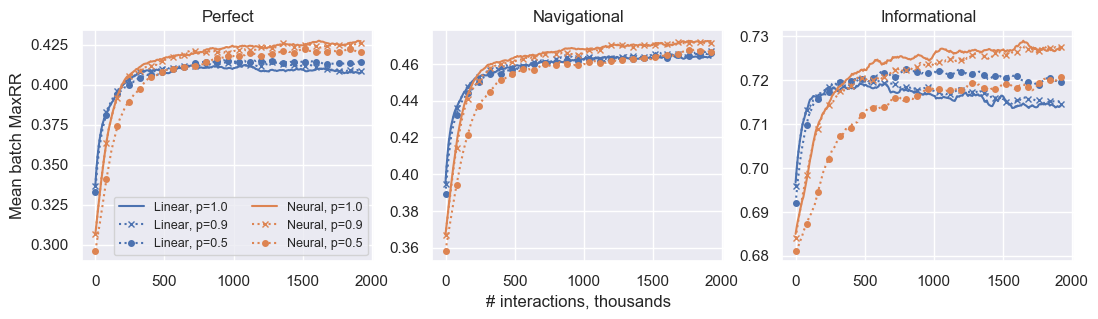
\includegraphics[width=15cm, height=3.5cm]{images/RQ1/mq2007_foltr_c2000_ps.png}
		\caption{Mean batch MaxRR for MQ2007.}
		\label{fig:mq2007-rq1}
	\end{subfigure}
	\begin{subfigure}{1\textwidth}
		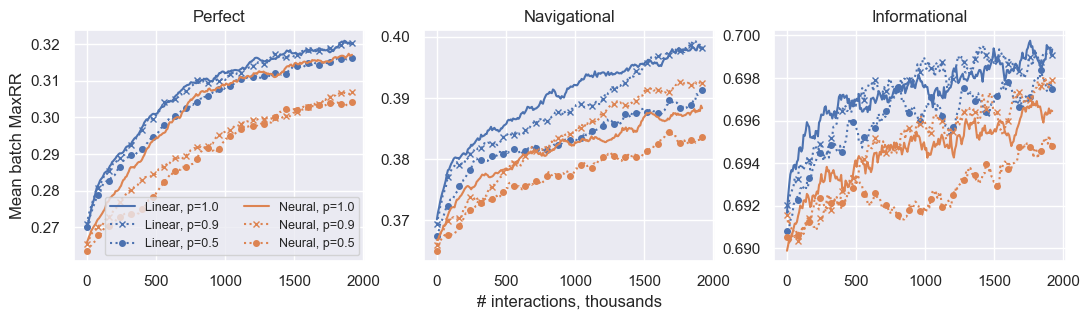
\includegraphics[width=15cm, height=3.5cm]{images/RQ1/mslr10k_foltr_c2000_ps.png}
		\caption{Mean batch MaxRR for MSLR10k}
		\label{fig:mslr10k-rq1}
	\end{subfigure}
	\begin{subfigure}{1\textwidth}
		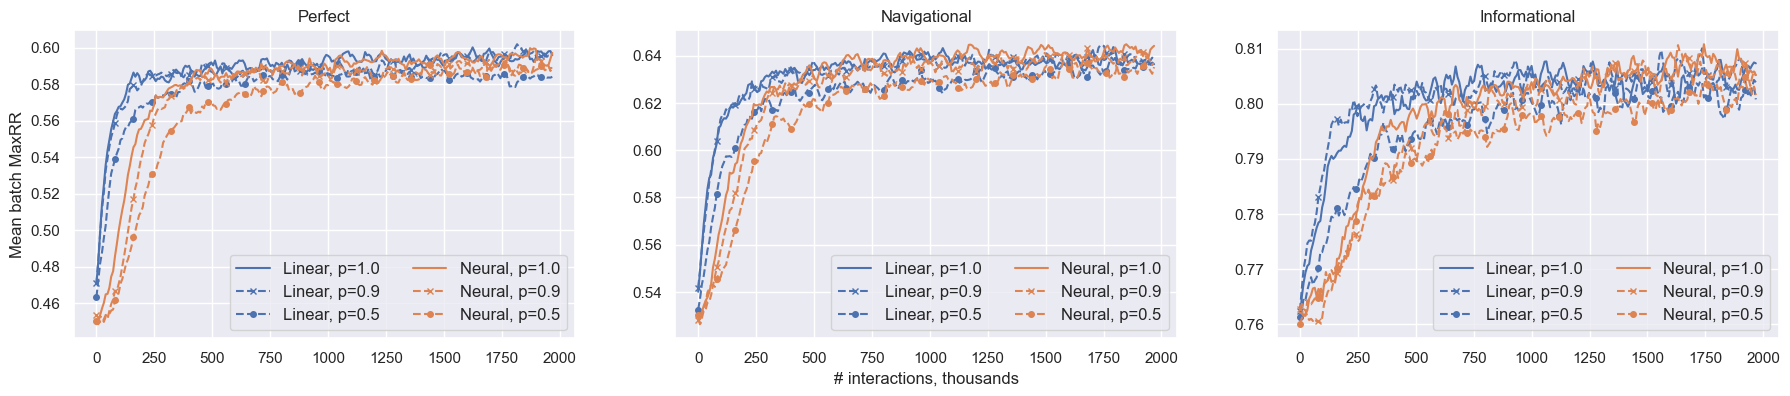
\includegraphics[width=15cm, height=3.5cm]{images/RQ1/yahoo_foltr_c2000_ps.png}
		\caption{Mean batch MaxRR for Yahoo.}
		\label{fig:yahoo-rq1}
	\end{subfigure}
	\caption{Results for RQ1: performance of FOLTR-ES across datasets.}
\end{figure}

Figure~\ref{fig:mq2007-rq1} reports the results obtained by FOLTR-ES on the MQ 2007 dataset\footnote{Similar results were obtained for MQ 2008 and are omitted for space reasons.} with respect to the three click models considered, various settings for the privacy preservation parameter $p$, and the two FOLTR-ES methods (linear and neural). Our results fully replicate those of Kharitonov~\cite{kharitonov2019federated} and indicate the following findings: (1) FOLTR-ES allows for the iterative learning of effective rankers; (2) high values of $p$ (lesser privacy) provide higher effectiveness; 
(3) the neural ranker is more effective than the linear ranker when $p \rightarrow 1$ (small to no privacy), while the linear model is equivalent, or better (for informational clicks) when $p=0.5$. 

However, not all these findings are applicable to the results obtained when considering MSLR-WEB10K and Yahoo, which are displayed in Figures~\ref{fig:mslr10k-rq1} and~\ref{fig:yahoo-rq1}. In particular, we observe that (1) the results for MSLR-WEB10K (and to a lesser extent also for Yahoo) obtained with the informational click model are very unstable, and, regardless of the click model, FOLTR-ES requires more data than with MQ 2007/2008 to arrive at a stable performance, when it does; (2) the neural ranker is less effective than the linear ranker, especially on MSLR-WEB10K. We believe these findings are due to the fact that query-document pairs in MSLR-WEB10K and Yahoo are represented by a larger number of features than in MQ2007/2008. Thus, more data is required for effective training, especially for the neural model; we also note that FOLTR-ES is largely affected by noisy clicks in MSLR-WEB10K. 

%In the previous work, FOLtR-ES is conducted on MQ2007 and MQ2008 datasets~\cite{kharitonov2019federated}. To further study if the algorithm can achieve similar ranking performance on other publicly available LTR datasets. We perform experiments on MSLR-WEB10K dataset using same parameters chosen by~\cite{kharitonov2019federated}, using antithetic variates and setting $B = 4$. 

%Unlike MQ2007 and MQ2008 datasets, FOLtR-ES performed on MSLR-WEB10K shows an opposite finding: the neural ranker dose not consistently perform better that the linear ranker. And for MSLR-WEB10K, FOLtR-ES takes more times on updating the ranker till it achieves the stable performance, which might be caused by larger training queries in MSLR-WEB10K. Figure \ref{fig: mq2007-rq1-1.0}\ref{fig: mslr-rq1-1.0}\ref{fig: mq2007-rq1-0.5}\ref{fig: mslr-rq1-0.5} show the mean batch MaxRR averaged on five data splits in MQ2007 and MSLR-WEB10K with the three click models.




%(Figures lack legend)
%\begin{figure}[H]
%	\centering
%	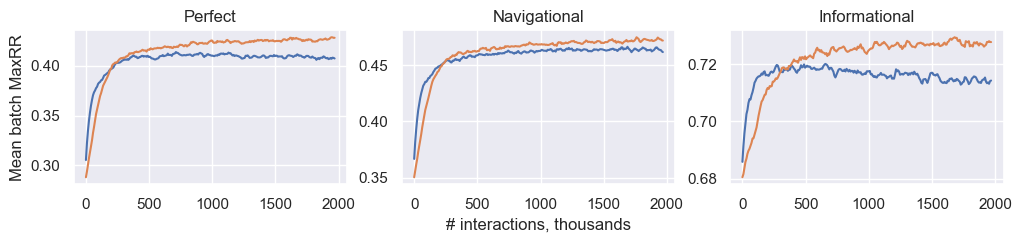
\includegraphics[width=15cm, height=3.5cm]{mq2007_foltr_c2000_p1.0.png}
%	\caption{Mean batch MaxRR for MQ2007 (2000 clients and $p = 0.9$)}
%	\label{fig: mq2007-rq1-1.0}
%\end{figure}
%\begin{figure}[H]
%	\centering
%	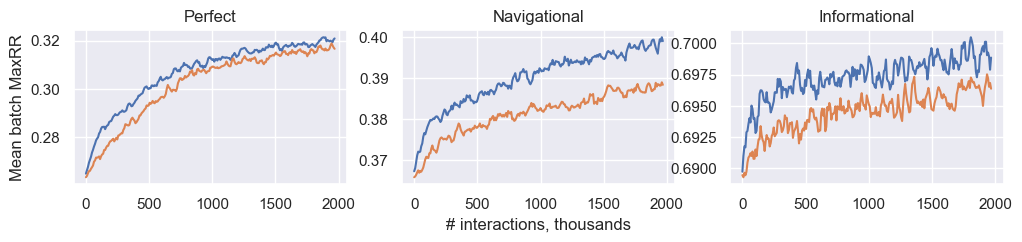
\includegraphics[width=15cm, height=3.5cm]{mslr10k_foltr_c2000_p1.0.png}
%	\caption{Mean batch MaxRR for MSLR-WEB10K (2000 clients and $p = 0.9$)}
%	\label{fig: mslr-rq1-1.0}
%\end{figure}
%
%\begin{figure}[H]
%	\centering
%	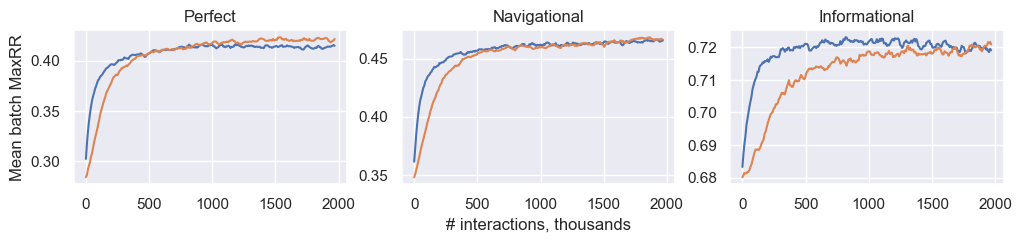
\includegraphics[width=15cm, height=3.5cm]{mq2007_foltr_c2000_p0.5.png}
%	\caption{Mean batch MaxRR for MQ2007 (2000 clients and $p = 0.5$)}
%	\label{fig: mq2007-rq1-0.5}
%\end{figure}
%\begin{figure}[H]
%	\centering
%	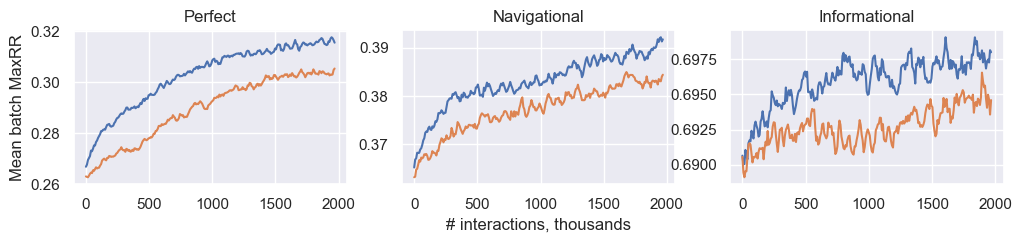
\includegraphics[width=15cm, height=3.5cm]{mslr10k_foltr_c2000_p0.5.png}
%	\caption{Mean batch MaxRR for MSLR-WEB10K (2000 clients and $p = 0.5$)}
%	\label{fig: mslr-rq1-0.5}
%\end{figure}

\subsection{RQ2: Effect of number of clients on FOLTR-ES}
%To answer RQ1, we perform experiments on MSLR-WEB10K dataset with the same FOLtR-ES setup
%Reproducing FOLtR-ES on other datasets

For answering RQ2 we vary thee number of clients involved in FOLTR-ES; we investigate the values \{50, 1,000, 2,000\}. Kharitonov~\cite{kharitonov2019federated} used 2,000 in the original experiments, and the impact of the number . To be able to fairly compare results across number of clients, we fixed the total number of ranker updates to 2,000,000; we also set $B = 4$ and vary the privatization parameter $p$ in \{0.5, 0.9, 1.0\}. We perform these experiments on all three datasets considered in this paper, but we omit to report results for Yahoo due to space limitations. 


\begin{figure}[t]
	\centering
	\begin{subfigure}{1\textwidth}
		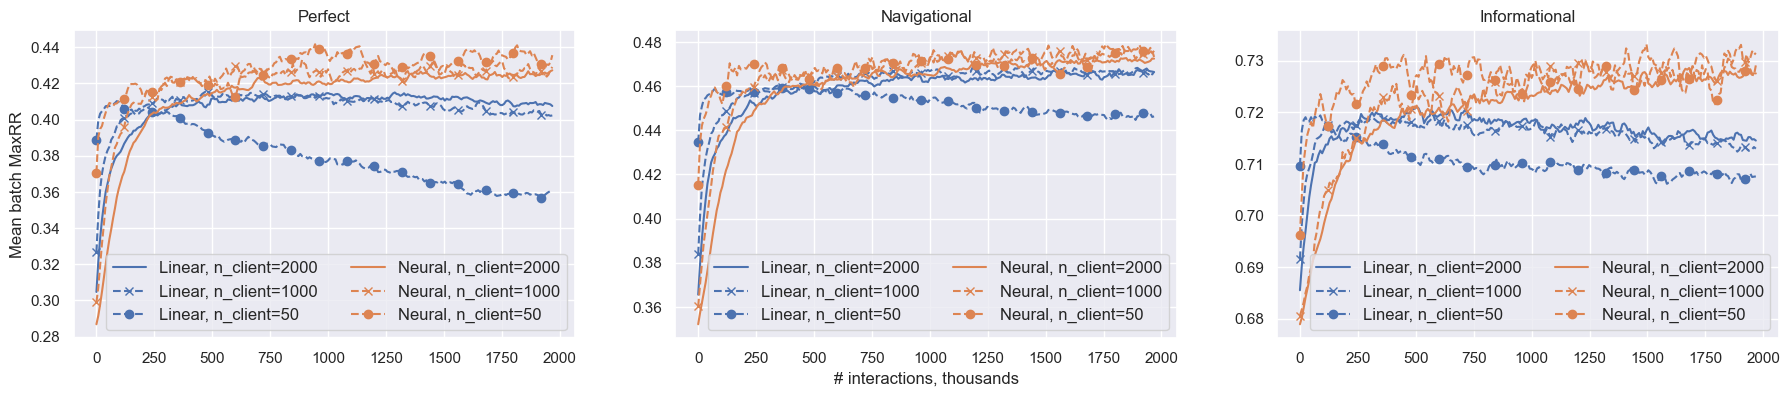
\includegraphics[width=15cm, height=3.5cm]{images/RQ2/mq2007_foltr_client_both_p0.9.png}
		\caption{Mean batch MaxRR for MQ2007.}
		\label{fig:mq2007-rq2}
	\end{subfigure}
	\begin{subfigure}{1\textwidth}
		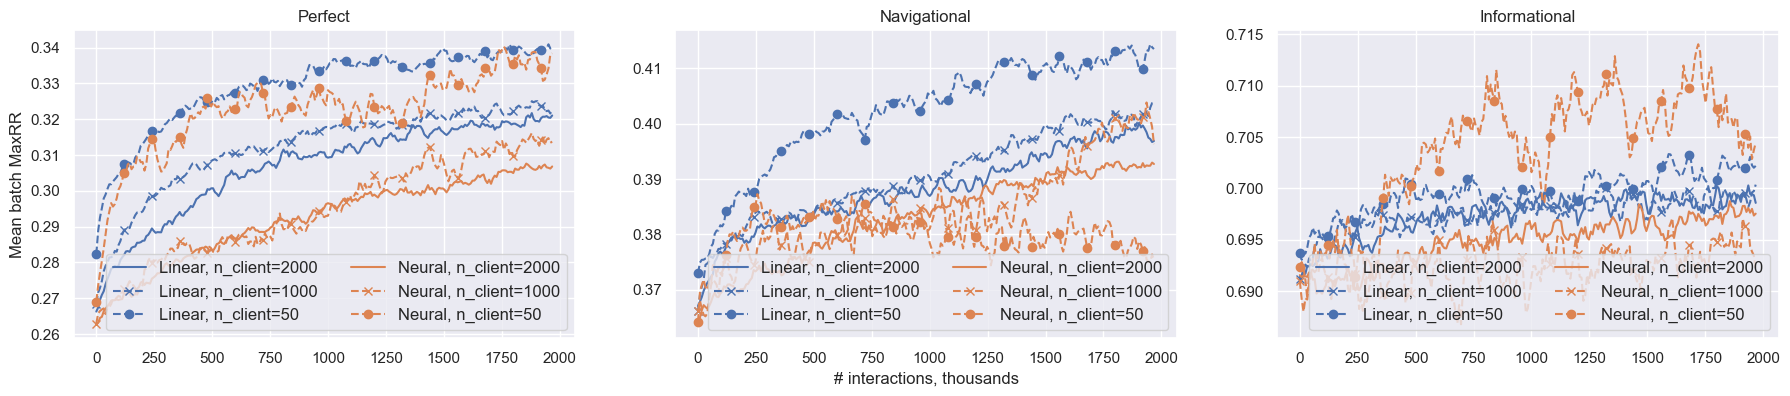
\includegraphics[width=15cm, height=3.5cm]{images/RQ2/mslr10k_foltr_client_both_p0.9.png}
		\caption{Mean batch MaxRR for MSLR10k}
		\label{fig:mslr10k-rq2}
	\end{subfigure}
	\caption{Results for RQ2: performance of FOLTR-ES with respect to number of clients. \label{fig:RQ2}} 
\end{figure}


The results of these experiments are reported in Figure~\ref{fig:RQ2}, and they are mixed. For MQ2007, the number of clients have little effect on the neural ranker used in FOLTR-ES, although when informational clicks are provided this ranker is less stable, although often more effective, if very few clients (50) are used. Having just 50 clients, instead, severally hits the performance of the linear ranker, when compared with 1,000 or 2,000 clients. The findings on MSLR10k, however, are different. In this dataset, a smaller number of clients (50), is generally better than larger numbers, both for linear and neural ranker. An exception to this is when considering navigational clicks: in this case the linear ranker obtains by far thee best performance with a small number of clients, but the neural ranker obtains the worst performance. This suggest that the number of clients greatly affects FOLTR-ES: but trends are not consistent across click types and datasets. 


%To study the influence of number of clients, we perform experiments on MQ2007 and MSLR-WEB10K datasets. We vary the number of clients across \{50, 1000, 2000\} but set the fixed total updating times to 2000000 and set $B = 4$. We also set the privatization parameter $p$ across \{0.5, 0.9, 1.0\}.

%Our experiments show that little clients number will reduce the performance in the linear ranker. But for the neural ranker, the difference is minor.

%\begin{figure}[H]
%	\centering
%	\includegraphics[width=16cm, height=8cm]{v0_mq2007_foltr_clients_p09.png}
%	\caption{Mean batch MaxRR for MQ2007 with different client number}
%	\label{fig: mq2007clients}
%\end{figure}
%\begin{figure}[H]
%	\centering
%	\includegraphics[width=15cm, height=3.5cm]{mq2007_foltr_client_linear_p09.png}
%	\caption{Mean batch MaxRR for MQ2007 with different client number (linear ranker and $p = 0.9$)}
%	\label{fig: mq2007-rq2-0.9}
%\end{figure}

\subsection{RQ3: Comparing FOLTR-ES to state-of-the-art OLTR methods}
The original study of FOLTR-ES did not compared the method with non-federated OLTR approaches. To contextualise the performance of FOLTR-ES and to understand the trade-off between privacy and performance done when designing FOLTR-ES, we compare this method with the current state-of-the-art OLTR method, the Pairwise Differentiable Gradient Descent (PDGD)~\cite{oosterhuis2018differentiable}. For fair comparison, we set the privatization parameter $p=1$ (lowest privacy) and the number of clients to 2,000. In addition note that in normal OLTR settings, rankers are updated after each user interaction: however in FOLTR-ES, rankers are updated in small batches. For fair comparison, we adapt PDGD to be updated in batch too. Instead of updating the ranker after each interaction (batch size 1), we accumulate gradients computed on the same batch size as for FOLTR-ES. Specifically, with 2000 clients for FOLTR-ES, the batch size of each update is 8,000 iterations (4 x 2,000). We then compute the updated gradients for PDGD on 8,000 interactiond too. %Note, the number of updates after 2m user interaction now becomes 2m/8000 = 250.
We perform these experiments on all three datasets considered in this paper, but we omit to report results for Yahoo due to space limitations. 

\begin{figure}[t]
	\centering
	\begin{subfigure}{1\textwidth}
		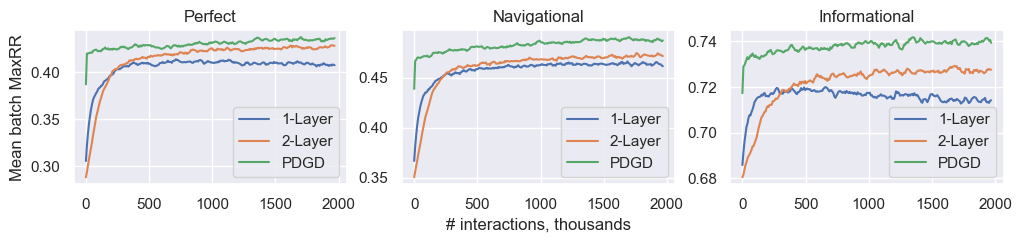
\includegraphics[width=15cm, height=3.5cm]{images/RQ3n4/mq2007_foltr_PDGD_mrr_c2000_p1.0}
		\caption{Mean batch MaxRR for MQ2007.}
		\label{fig:mq2007-rq3}
	\end{subfigure}
	\begin{subfigure}{1\textwidth}
		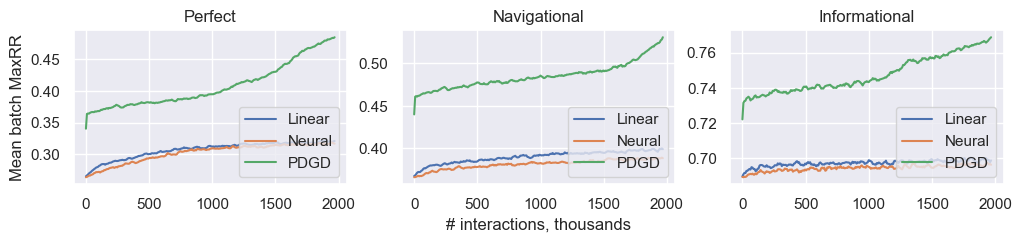
\includegraphics[width=15cm, height=3.5cm]{images/RQ3n4/mslr10k_foltr_PDGD_mrr_c2000_p1.0.png}
		\caption{Mean batch MaxRR for MSLR10k}
		\label{fig:mslr10k-rq3}
	\end{subfigure}
	\caption{Results for RQ3: performance of FOLTR-ES and PDGD across datasets. \label{fig:RQ3}} 
\end{figure}

Results are shown in Figure~\ref{fig:RQ3}: regardless of linear or neural ranker, FOLTR-ES is less effective than PDGD. The gap in performance is greater in larger datasets like MSLR10k and Yahoo (not shown) than in the smaller MQ2007/2008. This gap becomes even bigger, especially for the first iterations, if the PDGD ranker was updated after each iteration (not shown here), rather than after a batch has been completed. This highlights that FOLTR-ES has the merit of being the first privacy preserving federated OLTR approach available; however, more work is needed to improve the performance of FOLTR based methods so as to close the gap between privacy-oriented approaches and centralise approaches that do not consider user privacy.

%In order to further study the ranking quality, especially users' experience in FOLtR-ES, we perform experiments on comparing FOLtR-ES with the current state-of-the-art OLTR methods. In this section, we choose Pairwise Differentiable Gradient Descent (PDGD) models as baselines. For a fair comparation, we set up the privacy probability $p = 1$ (lowest privacy) in FOLtR-ES. We perform experiments on MQ2007 and MSLR-WEB10K datasets with simulating 2000 clients.

%Based on the experiment results, we can see FOLtR-ES still lags behind OLTR methods in terms of the ranking performance. As the ranking quality is an essential metric for web search engines, future work can be extend to improving ranking performance and in the meantime, protecting users' privacy.

%\begin{figure}[H]
%	\centering
%	\includegraphics[width=16cm, height=8cm]{v0_mq2007_foltr_vs_pdgd_2000clients_p10.png}
%	\caption{Mean batch MaxRR for MQ2007 with 2000 clients and $p = 1$}
%	\label{fig: mq2007-v0-baseline}
%\end{figure}
%
%\begin{figure}[H]
%	\centering
%	\includegraphics[width=16cm, height=8cm]{v0_mslr_foltr_vs_pdgd_2000clients_p10.png}
%	\caption{Mean batch MaxRR for MSLR-WEB10K with 2000 clients and $p = 1$}
%	\label{fig: mslr-v0-baseline}
%\end{figure}
%
%\begin{figure}[H]
%	\centering
%	\includegraphics[width=15cm, height=3.5cm]{mq2007_foltr_PDGD_mrr_c2000_p10.png}
%	\caption{Mean batch MaxRR for MQ2007 with two FOLtR-ES ranker(2000 clients and $p = 1$) and PDGD baselines}
%	\label{fig: mq2007-rq3}
%\end{figure}


\subsection{RQ4: Extending FOLtR-ES to other quality metric}


To study the generalisation of FOLtR-ES to other common OLTR evaluation metrics, we use Discounted Cumulative Gain (DCG) to evaluate the users' experience in each interaction. We also compute NDCG@10 with the relevance labels to evaluate the central ranker with test data as we want to explore the stability of  performance in FOLtR-ES.

In terms of nDCG evaluation, although FOLtR-ES achieves decent performance (with nDCG exceed 0.4 except for $Informational$ model), it still falls behind the PDGD baselines.

%\begin{figure}[H]
%	\centering
%	\includegraphics[width=15cm, height=3.5cm]{mq2007_foltr_PDGD_ndcg_c2000_p10.png}
%	\caption{Mean batch MaxRR for MQ2007 with(2000 clients and $p = 1$)}
%	\label{fig: mq2007-rq4}
%\end{figure}


(offline performance (NDCG) for different instantiations of CCM)
\section{Related Work}

Learning to rank (LTR) consists of the application of supervised machine learning techniques to learn a ranking function from a set of labelled query-document pair examples, represented by features. A key limitation of LTR is the reliance on explicit relevance annotations (labels), which require substantial effort and cost to collect~\cite{DBLP:journals/corr/QinL13,DBLP:journals/jmlr/ChapelleC11}. Editorial labelling also poses ethical issue when needing labels for private data~\cite{wang2016learning}, e.g., emails; in addition user preferences may not agree with that of annotators~\cite{sanderson2010test} and these labels cannot reflect evolving user preferences and search intents~\cite{lefortier2014online}.

The use of implicit feedback in the form of, e.g., clicks has been suggested as a way to go beyond the above limitations~\cite{joachims2002optimizing}; this is the type of signal that the methods studied in this paper consider. 
This setting however presents a number of challenges: clicks are affected by a number of biases and noise, e.g., position bias and noisy clicks~\cite{guan2007eye,joachims2017unbiased,pan2007google}. Approaches that exploit click feedback can be divided into counterfactual learning to rank (CLTR)~\cite{joachims2017unbiased} and online learning to rank (OLTR) \cite{yue2009interactively}. CLTR relies on historical click through logs, treated as pure binary relevance labels, and commonly \textit{inverse propensity scoring} (IPS) is used to re-weight clicks to minimise the impact of biases. Rankers are then trained in an offline manner and deployed online after training. 
OLTR instead, interactively updates rankers after each user interaction, in an online manner, and rankers explicitly manipulate SERPs to guide the learning process. This is the setup we consider in this paper, where rankers are iteratively updated in an online fashion following user interactions. A key aspect of OLTR is that the online interventions performed by rankers to guide the learning process carry the risk of displaying non optimal SERPs directly to the user, thus hurting user experience. It is important then for OLTR to rapidly learn a high quality ranker so as to not displaying low quality SERPs to a large number of users.

Little attention has been put on the fact that OLTR requires the search engine to monitor and collect user behaviour, thus not being appropriate when users want to preserve their privacy. In fact, current OLTR methods consider a central server that produces SERPs, collects queries and implicit user feedback, and updates a central ranker. An exception is the work of Kharitonov~\cite{kharitonov2019federated}, considered in this paper, that instead exploits federate learning to de-centralise the collection of user data and computation of gradient updates to the ranker; a central server is still required, but this only observes the federated gradient updates, which are then applied to the central ranker which is then distributed to the clients at each update iteration (more details in Section~\ref{sec:method}). Federated (machine) learning was recently introduced by Konecny et al.~\cite{DBLP:journals/corr/KonecnyMRR16,DBLP:journals/corr/KonecnyMYRSB16}; in this framework models are learnt based on datasets distributed across different locations (clients) without the need to share the actual data, and with mechanisms to guarantee data leakage~\cite{yang2019federated}. 
Privacy preservation is a topic of growing interest in information retrieval, with related workshops and tutorials being held in relevant venues~\cite{yang2016privacy,yang2017differential}, but its main focus so far has been on query log anonymisation and privacy-preservation when sharing logs~\cite{cooper2008survey,korolova2009releasing,zhang2016anonymizing}, rather than on integrating privacy preservation mechanisms within the ranking algorithms, as the work of Kharitonov instead does~\cite{kharitonov2019federated}.

%This section gives a brief overview of traditional LTR, OLTR and federated learning. 
%
%\subsection{Offline Learning to Rank}
%The core of Learning to Rank (LTR) is to train a ranking model using Machine Learning methods.
%
%\subsection{Online Learning to Rank}
%Main challenges in online learning to rank problem are: (a) noise and biases of user interactions, (b) non-continuous metrics for optimization.
%
%OLTR updates the ranker through user's online feedback, more specifically, user's click data. Unlike traditional LTR methods, OLTR doesn't need human-annotated data, which is expensive and time-consuming to create. Besides, human-annotated data can not always represent true preference of users. Traditional LTR methods are more suitable in situation where one ranking list fits all users. In a continuously developing world, people's preference and answers to one search query may change or differ from other's. OLTR provides a better way to learning from users' feedback in order to improve users' experience and ranking effectiveness.

%\subsection{Federated Machine Learning}
%
%Federated Machine Learning aims to solve two main challenges existing in today's artificial intelligence research: (a) data existing in the form of isolated islands, (b) the growing concern for data privacy and security~\cite{yang2019federated}. 
%
%The concept of Federated Learning was first proposed by Google in 2016~\cite{DBLP:journals/corr/KonecnyMRR16,DBLP:journals/corr/KonecnyMYRSB16}. The first Federated Learning algorithm is Federated Averaging~\cite{mcmahan2016federated}. In early year's research, the Federated Learning aims to train Machine Learning models using data from multiple data source while preventing data leakage. 



%Privacy preservation in IR~\cite{yang2016privacy,yang2017differential,cooper2008survey,korolova2009releasing,zhang2016anonymizing}

\section{Conclusions}

We set to explore 4 research questions. RQ1 aimed to investigate the generalisability of the original results obtained  by FOLTR-ES on the MQ2007/2008 dataset to other dataset used in current OLTR practice. Our reproducing experiments on MQ2007/2008 show the consistently similar findings with the original work. However, in terms of larger LTR datasets (MSLR-WEB10K and Yahoo datasets), the neural ranker is less effective than the linear ranker, especially on MSLR-WEB10K, which shows FOLtR-ES needs more data to achieve effective training on those datasets with larger number of features.
RQ2 aimed to investigate the effect varying the number of clients involved in FOLTR-ES has on the effectiveness of the method. We set the total times of interaction to a fix number and discover the ranking quality in terms of different number of clients in online simulation. Our experiments show that little clients number harm the performance in the linear ranker. But for the neural ranker, the difference is minor.
RQ3 aimed to compare FOLRT-ES with current OLTR state-of-the-art methods to understand the gap required to be paid for maintaining privacy. Our findings suggest that FOLtR-ES lags behind the OLTR baseline in terms of ranking performance
RQ4 aimed to investigate the generalisability of the original results obtained for FOLTR-ES to common evaluation practice in OLTR. \todo{Our findings suggest that ...}

\makeatletter
\renewcommand{\@biblabel}[1]{\hfill #1.}
\makeatother

\subsubsection*{Acknowledgements.}


\bibliographystyle{splncs04}
\bibliography{ecir2021-foltr-reproducibility}


%\end{thebibliography}

\end{document}

